\documentclass{VUMIFInfMagistrinis}
\usepackage{algorithmicx}
\usepackage{algorithm}
\usepackage{algpseudocode}
\usepackage{amsfonts}
\usepackage{amsmath}
\usepackage{bm}
\usepackage{color}
\usepackage{listings}
\usepackage{multirow}
\usepackage{graphicx}


\university{Vilniaus universitetas}
\faculty{Matematikos ir informatikos fakultetas}
\department{Informatikos katedra}
\papertype{Magistro baigiamasis darbas}
\title{Biografinių užklausų apdorojimas paskirstytose biometrinio identifikavimo sistemose}
\titleineng{Biographic Query Processing in Distributed Biometric Identification Systems}
\author{Rytis Karpuška}
\supervisor{prof. habil. dr. Mindaugas Bloznelis}
\reviewer{}
\date{Vilnius – \the\year}

\setmainfont{Palemonas}
\bibliography{bibliografija}

\begin{document}
\maketitle
%\sectionnonumnocontent{Santrauka}
%TODO: parašyti santrauką kai bus pakankamai darbo atlikta, kad būtų ką "sutraukti"
%
%\raktiniaizodziai{daugiamatė paieška, grupavimas, apdorojimas partijomis}
%
%\sectionnonumnocontent{Summary}
%TODO: parašyti santrauką kai bus pakankamai darbo atlikta, kad būtų ką "sutraukti"
%
%\keywords{multidimensional search, clustering, batch processing}

\tableofcontents


%Įvade aprašomi darbo tikslai, nurodomas temos aktualumas, aptariamos teorinės
%darbo prielaidos bei metodologija, apibrėžiamas tiriamasis objektas,
%apibūdinami su tema susiję literatūros ar kitokie šaltiniai, temos analizės
%tvarka, darbo atlikimo aplinkybės, pateikiama žinių apie naudojamus
%instrumentus (programas ir kt.). Rekomenduojama įvado apimtis 3-4 puslapiai.

\sectionnonum{Įvadas}

% Kas yra biometrines identifikavimo sistemos
Kiekvieno žmogaus kūnas turi aibę savybių, kurios gali unikaliai jį identifikuoti (pvz.: pirštų atspaudai).
Šių savybių egzistavimas davė pagrindą {\it biometrinėms identifikavimo sistemoms}.
Biometrinio identifikavimo sistema yra tokia sistema, kuri geba palyginti kandidato biometrinius įrašus su aibe kitų biometrinių įrašų ir atrinkti kurie iš jų galėtų priklausyti tam pačiam žmogui.
Tokiose sistemose yra poreikis gebėti atrinkti poaibį visų žinomų biometrinių įrašų, su kuriais būtų atliekamas biometrinis palyginimas.

% Kas yra biografinė užklausa ir biografiniai atributai?
Šio poaibio sudarymas bei biometrinių įrašų palyginimas vadinamas {\it biografinių užklausų apdorojimu}.
Atrinkimas yra vykdomas pagal {\it biografinius atributus}.
Su kiekvienu biometriniu įrašu siejama aibė biografinių atributų (žr.: \ref{tab:exampleGallery} lentelę).
Biografinis atributas tai yra papildomas duomuo (pvz.: žmogaus amžius, lytis, šalis kurioje gyvena ir pan.), kuris gali būti:
\begin{itemize}
\item skaitinio tipo
\item simbolių eilutės (ang.: string) tipo
\end{itemize}

Su biografine užklausa yra siejamas predikatas, pagal kurį yra įvertinama kiekvieno biometrinio įrašo biografinių atributų aibė siekant sudaryti įrašų poaibį palyginimams.

\begin{table}[H]\footnotesize
	\centering
	\begin{tabular}{|c|c|c|c|}
		\hline
		\multirow{2}{*}{{\bf Subjektas}} & \multirow{2}{*}{{\bf Biometriniai duomenys}} & \multicolumn{2}{|c|}{{\bf Biografiniai atributai}}  \\ \cline{3-4}
		& & {\bf Piršto atspaudo pozicija} & {\bf Subjekto amžius} \\
		\hline
		Jonas  & biometrinis įrašas & Kairys nykštys  & 25 \\ \cline{2-4}
		       & biometrinis įrašas & Dešinys nykštys & 25 \\
		\hline
		Mindaugas & biometrinis įrašas & Kairys nykštys  & 35 \\ \cline{2-4}
		          & biometrinis įrašas & Dešinys nykštys & 35 \\
		\hline
	\end{tabular}
	\caption{Pavyzdiniai biometrinės identifikavimo sistemos duomenys}
	\label{tab:exampleGallery}
\end{table}

% Biographic schema
Visų biografinių atributų prasmių aibė vadinama {\it biografine schema}. Pavyzdžiui \ref{tab:exampleGallery} lentelę atitinkanti biografinė schema būtų \{„Piršto atspaudo pozicija“, „Subjekto amžius“\}.

\paragraph{Biografinių užklausų predikatai}

Vykstant biografinės užklausos apdorojimui, su ja susietas predikatas apsprendžia aibę biometrinių įrašų, kurie bus lyginami su kandidato biometriniu įrašu.
Į šią aibę patenka tik tie biometriniai įrašai, kurių biografinių atributų aibė tenkina užklausos predikatą.
Predikatai sistemai yra aprašomi specialia tam skirta kalba.
\ref{tab:queryBNF} lentelė pateikia šios kalbos BNF formą.

\begin{table}[H]\footnotesize
	\centering
	\begin{tabular}{|l c l|}
		\hline
		predikatas                    & ::= & <išraiška> \\
		išraiška                      & ::= & <vienaris operatorius> <operandas> | \\
									  &     & \multicolumn{1}{l|}{<operandas> <dvinaris operatorius> <operandas> |} \\
									  &     & \multicolumn{1}{l|}{"(" <išraiška> ")" |} \\
									  &     & \multicolumn{1}{l|}{ <atributo vardas> <sąrašo operatorius> <sąrašas>} \\
		operandas                     & ::= & <išraiška> | <atributo vardas> | "'" <skaičius> "'" | "'" <žodis> "'" \\
		vienaris operatorius          & ::= & <neprivalomas tarpas> "NOT" <neprivalomas tarpas> \\
		dvinaris operatorius          & ::= & <neprivalomas tarpas> <dvinario operatoriaus ženklas> <neprivalomas tarpas> \\
		dvinario operatoriaus ženklas & ::= & ">" | ">=" | "<" | "<=" | "=" | "<>" | "AND" | "OR" \\
		sąrašo operatorius            & ::= & <neprivalomas tarpas> "IN" <neprivalomas tarpas> \\
		sąrašas                       & ::= & "(" <sąrašo elementai> ")" \\
		sąrašo elementai              & ::= & <sąrašo elementas> | <sąrašo elementas> "," <sąrašo elementai> \\
		sąrašo elementas              & ::= & "'" <žodis> "'" | "'" <skaičius> "'" \\
		atributo vardas               & ::= & <neprivalomas tarpas> <žodis> <neprivalomas tarpas> \\
		neprivalomas tarpas           & ::= & "" | " " <neprivalomas tarpas> \\
		žodis                         & ::= & <raidė> | <žodis> <raidė> | <žodis> <skaičius> \\
		skaičius                      & ::= & "0" | "1" | "2" | "3" | "4" | "5" | "6" | "7" | "8" | "9" \\
		raidė                         & ::= & "A" | "B" | "C" ... "Z" | "a" | "b" | "c" ... "z"  \\
		\hline
	\end{tabular}
	\caption{Biografinės užklausos predikato aprašymo kalbos BNF forma}
	\label{tab:queryBNF}
\end{table}

Keletas užklausos predikato aprašymo pavyzdžių pateikiama \ref{tab:queryExamples} lentelėje.

\begin{table}[H]\footnotesize
	\centering
	\begin{tabular}{|c|l|}
		\hline
		{\bf Užklausos predikato aprašymas} & {\bf Užklausos prasmė} \\
		\hline
		Amzius > '18' & Visi suaugę žmonės\\
		\hline
		Amzius > '18' AND Miestas IN ('Vilnius', 'Kaunas', 'Klaipeda') & Visi suagę vilniečiai, kauniečiai ir klaipėdiečiai \\
		\hline
		NOT (Miestas = 'Vilnius' AND Amzius > '18') & Visi žmonės išskyrus suaugusius vilniečius \\
		\hline
	\end{tabular}
	\caption{Užklausų predikato aprašymo pavyzdžiai.}
	\label{tab:queryExamples}
\end{table}

% maybe some more comments?



% Sistemos greičio svarba, paminim, kad dirbsim su Neurotechnology akseleratorium
\paragraph{Sistemos greitis}

Biometrinio identifikavimo sistemos darbo greitis yra labai aktuali sistemos savybė.
Kartais \cite{NeurotechnologyDRCDedublicationProject} \cite{NeurotechnologyVenezuelaDedublicationProject} tai yra pagrindinis faktorius apsprendžiantis projekto trukmę.
Šiame darbe bus nagrinėjami metodai padedantys optimizuoti bendrą UAB „Neurotechnolgy“ biometrinės identifikavimo sistemos \cite{NeurotechnologyMegamatcherAccelerator} darbo greitį vykdant biografines užklausas.

% Visa duomenų bazė RAM`e
Tipinės biografinės užklausos metu palyginimui yra atrenkama didelė dalis visų sistemai žinomų biometrinių įrašų.
Tai lėmė dizaino sprendimą saugoti visus sistemai žinomus biometrinius įrašus operatyviojoje kompiuterio ar serverio atmintyje darbo metu.

% Introducinam batch processingą ir blokus
UAB „Neurotechnology“ biometrinio palyginimo algoritmai yra optimizuoti siekiant pagerinti procesoriaus spartinančiosios atminties išnaudojimą.
Dėl šios priežasties biometriniai įrašai atmintyje laikomi optimizuojant atminties prieigos vientisumą.
Tačiau ribotas spartinančiosios atminties kiekis lemia, kad atminties prieigos vientisumo poveikis juntamas tik iki tam tikro, nuo konkretaus procesoriaus priklausančio, atminties bloko dydžio.
Tai lėmė, kad biometriniai įrašiai yra saugomi {\it biometrinių įrašų blokuose}.
Biometrinių įrašų blokas yra visų žinomų biometrinių įrašų poaibis saugomas vientisame atminties bloke.

Keletas svarbių biometrinių įrašų blokų savybių:
\begin{itemize}
\item Visų blokų dydžiai sistemoje yra vienodi.
\item Kiekvienas biometrinis įrašas yra saugomas tiktai viename bloke siekiant maksimizuoti bendrą sistemos biometrinių įrašų talpą.
\item Blokai gali turėti tuščių vietų.
\item Maksimalus blokų kiekis yra ribotas ir apsrendžiamas techninės įrangos.
\end{itemize}

Taip pat svarbu pastebėti tai, kad atliekant biometrinę identifikaciją biometrinio palyginimo operacijos yra vykdomos įrašų blokams, o ne pavieniams įrašams.
Todėl net jeigu bloke yra įrašų, kurie neatitinka biografinės užklausos predikato, su jais vistiek yra vykdomas biometrinis palyginimas, tačiau jie neįtraukiami į galutinius rezultatus.

%\begin{figure}[H]
%\begin{center}
%
\includegraphics[width=0.4\textwidth]{img/BiometricRecordBlocks.eps}
%\caption{Pavyzdiniai biometrinių įrašų blokai. \\ Čia taškai -- įrašai, o stačiakampiai -- blokai}
%\label{img:exampleGallery}
%\end{center}
%\end{figure}

\paragraph{Darbo tikslas}

Verta pastebėti, kad UAB „Neurotechnology“ biometrinės identifikavimo sistemos darbo korektiškumas nepriklauso nuo to kuriems blokams yra priskirami biometriniai įrašai.
Tačiau darbo greitis gali kisti drastiškai.
Todėl šiam darbui keliami tikslai:
\begin{enumerate}
	\item Surasti efektyvų metodą priskirti biometrinius įrašus blokams, minimizuojant vidutinį nereikalingų biometrinių palyginimų skaičių.
	\item Surasti efektyvų metodą atrinkti blokus, kurie turi biometrinių įrašų atitinkančių biografinės užklausos predikatą.
\end{enumerate}

Nereikalingų palyginimų skaičius bus vertinamas pagal šiuos matavimus:
\begin{itemize}
	\item Dalis visų blokų, kurie turi nors vieną biografinės užklausos predikatą atitinkantį įrašą. (siekiama minimizuoti).
	\item Dalis Bloko įrašų, kuri atitinka biografinės užklausos predikatą. (siekiama maksimizuoti).
	\item Tuščias vietas esančias blokuose. (siekiama minimizuoti).
\end{itemize}

Šio darbo metu bus analizuojama kokiomis savybėmis pasižymi dažniausiai pasitaikančios biografinės užklausos.
Vėliau bus vertinama kokią įtaką darbo greičiui turi blokų užpildymas, bei blokų įrašų atitikimas vidutiniam predikatui.
Tuomet bus ieškoma metodo, padedančio optimizuoti sistemos darbą pagal ankščiau įvardintus kriterijus.




%\section{Literatūros apžvalga}

Panaši problema į aptartąją įvade yra nemažai tyrinėjama duomenų bazių kontekste.
Čia minimizuojamas disko operacijų skaičius siekiant sumažinti duomenų bazės atsako laiką bei padidinti pralaidumą (apdorotų užklausų skaičių per laiko vienetą) \cite{garcia2000database}.
Panašiai kaip šiame darbe siekiama minimizuoti biometrinių įrašų blokų skaičių likusį po atmetimo etapo siekiant pagerinti sistemos \cite{NeurotechnologyMegamatcherAccelerator} pralaidumą.
Tuo tikslu yra naudojama duomenų struktūra, vadinama {\it duomenų indeksu}.
Jeigu duomenys yra daugiamačiai (vienas įrašas gali susidėti iš daugiau negu vienos reikšmės), tuomet indeksas tokiems duomenims vadinamas {\it daugiamačių duomenų indeksu}, o metodas pagal kurį šis indeksas yra sudaromas bei naudojamas {\it daugiamačių duomenų indeksavimo metodu}.

\subsection{Užklausų klasifikacija}

Šiame darbe palyginant indeksavimo metodus sistemoje \cite{NeurotechnologyMegamatcherAccelerator} siekiama apimti kiek galima daugiau užklausų klasių pagal Gaede ir Günther \cite{gaede1998multidimensional} pateikiamą daugiamačių užklausų klasifikaciją:
\begin{enumerate}
	\item Griežto atitikmens užklausa
	\item Taško užklausa
	\item Lango užklausa
	\item Regiono užklausa
	\item Apgaubiančioji užklausa
	\item Pilno regiono užklausa
	\item Kaimynų užklausa
	\item Artimiausio kaimyno užklausa
\end{enumerate}

Autorius duomenis ir užklausas nagrinėja $d$ dimensijų euklido erdvėje $E^d$.
Atskirus įrašus apibrėžia kaip objektus $o$ kurie gali turėti 0 ar daugiau papildomų atributų nesusijusių su erdve $E^d$ (pvz.: vardas, pavadinimas, amžius...), bei griežtai vieną atributą $o.G$, kuris apibūdina objekto $o$ padėtį erdvėje $E^d$.
Šis $o.G$ atributas yra aibė taškų, kuriuos objektas $o$ užima erdvėje $E^d$.
Objektams yra apibrėžiami operatoriai $=$, $\cap$, bei $dist(o_1, o_2)$.
Du objektai $o_1$ ir $o_2$ skaitomi lygiais $o_1 = o_2$ tada ir tik tada jeigu abiejų objektų užimamų taškų aibės $o_1.G$ ir $o_2.G$ sutampa.
Dviejų objektų $o_1$ ir $o_2$ sankirta $o_1 \cap o_2$ yra aibė taškų, kurie patenka ir į $o_1.G$ ir į $o_2.G$.
Ir galiausiai atstumas tarp dviejų objektų $o_1$ ir $o_2$ $dist(o_1, o_2)$ skaitomas mažiausias atstumas tarp bet kurių dviejų taškų esančių $o_1.G$ ir $o_2.G$ aibėse.



\subsubsection{Griežto atitikmens užklausa}
Griežto atitikmens užklausa yra tokia užklausa, kuri duotąjam objektui $o'$ erdvėje $E^d$ randa visus objektus, kurių erdvės sritys sutampa su duotąja:

\begin{equation}
	EMQ(g) = \{ o | o'.G = o.G \}
\label{eq:ExactMatchQuery}
\end{equation}

\subsubsection{Taško užklausa}
Taško užklausa yra tokia užklausa, kuri duotam taškui $p$ erdvėje $E^d$ randa visus objektus, kurie turi bendrų taškų:

\begin{equation}
	PQ(p) = \{ o | \{p\} \cap o.G = \{p\} \}
\label{eq:ExactMatchQuery}
\end{equation}

Žiūrėti priedą \ref{app:pointQuery}.

\subsubsection{Lango užklausa}
Lango užklausa, tai tokia užkausa, kuri duotiems $d$ intervalams $I^d = [l_1, u_1] \times [l_2, u_2] \times ... \times [l_d, u_d]$ (po vieną kiekvienai erdvės $E^d$ koordinačių ašiai) randa visus objektus $o$ kurie turi bendrų taškų:

\begin{equation}
	WQ(I^d) = \{ o | I^d \cap o.G \neq \emptyset \}
\label{eq:ExactMatchQuery}
\end{equation}

Verta pastebėti, kad lango užklausos atveju visos erdvės srities kraštinės yra lygegriačios erdvės $E^d$ koordinačių ašims.
Žiūrėti priedą \ref{app:windowQuery}.


\subsubsection{Regiono užklausa}
Regiono užklausa yra labai panaši į Lango užklausą, tačiau srities kraštinės gali būti laisvai pasirinktos, ir neturi būti lygegriačios koordinačių ašims.
Regiono užklausa randa visus objektus, kurie turi bendrų taškų su duotuoju objektu $o'$.

\begin{equation}
	IQ(g) = \{ o | o'.G \cap o.G \neq \emptyset \}
\label{eq:ExactMatchQuery}
\end{equation}
Žiūrėti priedą \ref{app:intersectionQuery}.

\subsubsection{Apgaubiančioji užklausa}
Apgaubiančioji užklausa yra tokia užklausa, kuri randa visus objektus $o$, kurių erdvės sritis $o.G$ pilnai apima pateiktąjį objektą $o'$:

\begin{equation}
	EQ(g) = \{ o | (o'.G \cap o.G) = o.G \}
\label{eq:ExactMatchQuery}
\end{equation}
Žiūrėti priedą \ref{app:enclosureQuery}.


\subsubsection{Pilno regiono užklausa}
Pilno regiono užklausa iš esmės yra priešinga apgaubiančiąjai.
Pilno regiono užklausa yra tokia užklausa, kuri randa visus objektus $o$, kurių erdvės sritis $o.G$ pilnai patenka į pateikatjį objektą $o'$:

\begin{equation}
	CQ(g) = \{ o | (o'.G \cap o.G) = o'.G \}
\label{eq:ExactMatchQuery}
\end{equation}
Žiūrėti priedą \ref{app:containmentQuery}.


\subsubsection{Kaimynų užklausa}
Kaimynų užklausa yra tokia užklausa, kuri pagal duotąjį objektą $o'$ suranda visus šio objekto kaimynus, t.y. objektus $o$ kurie turi bendrą kraštinę erdvėje $E^d$:

\begin{equation}
	AQ(g) = \{ o | (o'.G \cap o.G) \neq \emptyset \land o'.G\textdegree \cap o.G\textdegree = \emptyset \}
\label{eq:ExactMatchQuery}
\end{equation}

Čia $o.G\textdegree$ reiškia visus vidinius taškus, kurie priklauso sričiai $o.G$.
Žiūrėti priedą \ref{app:adjacencyQuery}.


\subsubsection{Artimiausio kaimyno užklausa}
Artimiausio kaimyno užklausa yra tokia užklausa, kuri duotam objektui $o'$ randa artimiausią kaimyną (verta pastebėti, kad šiuo atveju kaimynai gali ir neturėti bendrų kraštinių).

\begin{equation}
	NNQ(o') = \{ o | \forall o'' : dist(o'.G, o.G) \leq dist(o'.G, o''.G) \}
\label{eq:ExactMatchQuery}
\end{equation}




\subsection{Daugiamačių duomenų indeksavimo metodų klasifikacija}
Lu ir Ooi \cite{lu1993spatial}, Gaede ir Günther \cite{gaede1998multidimensional}, bei B{\"o}hm, Christian, Stefan, Daniel A \cite{bohm2001searching} apžvelgia įvairius daugiamačių duomenų indeksus, bei pateikia schemą padedančią suprasti jų istoriją (žiūrėti priedą \ref{app:multidimensionalIndexing}).

Autoriai šiuos metodus suskirsto į tris grupes:
\begin{itemize}
	\item Metodai paremti maišos funkcijomis.
	\item Hierarchiniai metodai.
	\item Metodai paremti erdvę užpildančiomis kreivėmis \cite{bader2012space}.
\end{itemize}



\subsubsection{Maišos funkcijomis paremti metodai daugiamačių duomenų indeksavimui}

% generic description
% basically hash tables where buckets are bloks in multidimensional space
% order preserving hashes
% pritaikymo pavyzdžiai

Verta pastebėti, kad dažnai maišos funkcijomis paremti metodai yra tinkami tik griežto atitikmens užklausoms \cite{nievergelt1981grid} \cite{tamminen1982excell}.
Todėl šiame darbe tokie metodai nebus įgyvendinami ir lyginami sistemoje \cite{NeurotechnologyMegamatcherAccelerator}.


\subsubsection{Hierarchiniai metodai daugiamačių duomenų indeksavimui}

Hierarchiniai daugiamačių duomenų indeksai yra paremti dvejetainiais ar aukštesnio atsišakojimo faktoriaus medžiais (trejetainiai, ketvirtainiai...) \cite{gaede1998multidimensional}.
Šie indeksai saugo įrašus ne po vieną, bet grupėmis.
Dažniausiai kiekviena grupė yra randama medžio lapuose (vadinama {\it duomenų viršūne}).
Vidinės viršūnės (vadinamos {\it indekso viršūnėmis}) yra naudojamos kaip kelrodžiai ieškant duomenų viršūnių.
Kiekviena indekso viršūnė nurodo visas duomenų viršūnes, kurios gali būti rastos šios indekso viršūnės pomedyje.

%TODO: image

Užklausų apdorojimas yra skaidomas į du etapus:
\begin{enumerate}
	\item Iteravimas medžiu.
	\item Įrašų filtravimas.
\end{enumerate}
Iteravimo medžiu etape, yra „prabėgamas“ medis nuo šaknies iki lapų ir atrenkamos visos duomenų viršūnės, kurios gali turėti įrašų atitinkančių užklausos kriterijus.
Filtravimo metu atrenkami įrašai esantys iteravimo etape atrinktose grupėse ir tenkinatys užklausos kriterijus \cite{brinkhoff1994multi} \cite{bohm2001searching}.
Verta pastebėti, kad sistemoje \cite{NeurotechnologyMegamatcherAccelerator} užklausų apdorojimo etapai yra labai panašūs.

\paragraph{Kd-medis}

Šiame darbe bus aptariamas biometrinių įrašų priskyrimo blokams metodas paremtas Kd-medžiu \cite{bentley1979multidimensional}.
Kd-medžių duomenys yra taškai $E^d$ erdvėje.
Kd-medis yra dvejetainis medis, kurio lapuose (duomenų viršūnėse) yra saugomi vienas ar daugiau $d$-mačių taškų.
Kiekviena vidinė medžio viršūnė (indekso viršūnė) dalina erdvę $E^d$ į dvi nepersidengiančias dalis.
Taškai patenkantys į vieną dalį patenka į kairyjį pomedį, o patenkantis į kitą dalį -- į dešinį pomedį (žr.: \ref{img:KdTreeExample} pav.).
Erdvės dalinimas į dvi dalis yra parenkamas taip: kiekvienai vidinei viršūnei yra parenkama koordinačių ašis (pvz.: $x$) ir reikšmė (pvz .: $5$).
Tuomet visi taškai, kurių $x$ koordinatės reikšmė yra mažesnė už parinktą reikšmę (pavyzdyje $[-\infty; 5)$), patenka į kairyjį pomedį, likę taškai (pavyzdyje $[5; \infty)$) -- į dešinį pomedį.
Nėra griežtai apibrėžta kokia koordinačių ašis ar reikšmė šioje ašyje turi būti parinkta kiekvienai viršūnei, todėl šiuo tikslu taikomos įvairios euristikos.

\begin{figure}[H]
\begin{center}
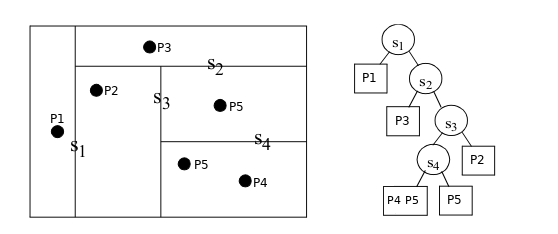
\includegraphics[width=0.7\textwidth]{img/KdTreeExample.png}
\caption{Kd-medžio pavyzdys.}
\label{img:KdTreeExample}
\end{center}
\end{figure}

Paveiksliuke \ref{img:KdTreeExample} pateikiamas Kd-medžio pavyzdys.
Čia kairėje -- šį medį atitinkanti erdvė $E^d$.
Taškai $P1$-$P5$ atitinka daugiamačius duomenis, o tiesės $S1$-$S4$ - erdvės $E^d$ padalijimus atitinkmai medžio viršūnėse $S1$ - $S4$.

Hierarchiniai metodai daugiamačių duomenų indeksavimui yra plačiai taikomi duomenų bazių \cite{bohm2001searching}, sensorių tinklų \cite{li2003multi}, paveiksliukų paieškoje \cite{silpa2008optimised}, privatumo \cite{hore2012secure} \cite{xiao2010differentially} ir kitose srityse.

\subsubsection{Erdvę užpildančiomis kreivėmis paremti metodai daugiamačių duomenų indeksavimui}

Kaip ir hierarchiniuose metoduose taip ir erdvę užpildančiomis kreivėmis paremtuose metoduose duomenys nagrinėjami kaip taškai euklido erdvėje $E^d$

Daugiamačiai duomenys neturi pilnos tvarkos, pagal kurią šalia esantys taškai būtų arti ir erdvėje $E^d$.
Dėl šios priežasties daugiamačių duomenų indeksavimo metodai yra sudėtingesni lyginant su vienmačiais \cite{gaede1998multidimensional} \cite{bohm2001searching}
Tačiau egzistuoja įvairiomis euristikomis paremtų pilnos tvarkos sudarymo metodų, kurie su nemaža tikimybe taip sudeda taškus.
Ši pilna tvarka yra vienmatė erdvė $E'^1$ kurią galima indeksuoti vienmačiais indeksavimo metodais (B-medžiu \cite{comer1979ubiquitous} RB-medžiu \cite{hanke1997relaxed} ir pan.).

Siekiant sudaryti tokią tvarką, $E^d$ erdvė suskirstoma į gardelę (į kiekvieną laukelį šioje gardelėje gali patekti nulis, vienas ar daugiau taškų).
Kiekvienam laukeliui šioje gardelėje yra priskiriamas unikalus skaičius pagal kurį laukeliai yra surikiuojami ir indeksuojami vienmačiais indeksavimo metodais.
Šie unikalūs skaičiai yra priskiriami pagal tai kokia tvarka erdvę užpildanti kreivė \cite{bader2012space} „prabėga“ pro laukelius.
Aptarsime dvi tokias kreives:
\begin{enumerate}
	\item Eilutinę kreivę.
	\item Z-kreivę.
\end{enumerate}

\paragraph{Eilutinė kreivė}

Eilutinė kreivė yra viena iš papraščiausių erdvę užpildančių kreivių.
Ji negali būti naudojama begalinėje erdvėje, todėl tarkime, kad $[L_i; U_i]$ yra erdvės $E^d$ ribos dimensijos $i$ atžvilgiu.
Eilutinė kreivė iš pradžių „prabėga“ visus taškus didėjimo tvarka $[x, L_2, ..., L_d]$, kur $x \in [L_1; U_1]$.
Paskui „prabėga“ $[x, L_2 + 1, ..., L_d]$, paskui $[x, L_2 + 2, ..., L_d]$ ir t.t. (žr.: \ref{img:RowWiseSpaceFillingCurve} pav.).

\begin{figure}[H]
\begin{center}
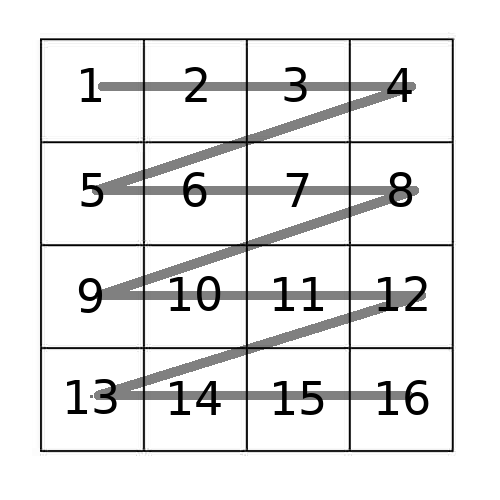
\includegraphics[width=0.3\textwidth]{img/RowWiseSpaceFillingCurve.png}
\caption{Eilutinės erdvę užpildančios kreivės pavyzdys.}
\label{img:RowWiseSpaceFillingCurve}
\end{center}
\end{figure}


Formaliai tvarka yra apibrėžiama sąryšio:
\begin{equation}
	p_1 < p_2 \text{ jeigu } RWSFC(p_1) < RWSFC(p_2)
\label{eq:RowWiseSFCComparison}
\end{equation}

Čia $p_1$ ir $p_2$ yra taškai erdvėje $E^d$, o $RWSFC(p)$:

\begin{equation}
	RWSFC(p) = 1 + \sum_{i=1}^{d} [(p_i - L_i) \prod_{j=0}^{i - 1}U_j - L_j]
\label{eq:RowWiseSFCValue}
\end{equation}

Čia daroma prielaida, kad $U_0 - L_0 = 1$.



\paragraph{Z-kreivė}

Daugiamačių duomenų indeksavimo metodų kontekste Z-kreivė yra viena iš populiariausių \cite{ramsak2000integrating}.
Z-kreivė visų pirmą visą erdvę $E^d$ padalina į dvi lygias sritis $p_0$ ir $p_1$ statmenai pirmai koordinačių ašiai.
Z-kreivė visus laukelius esančius srityje $p_0$ „prabėga“ pirmiau tų, kurie yra srityje $p_1$.
Sekančiame žingsnyje $p_0$ ir $p_1$ yra padalinamos į dvi lygias sritis $p_{00}$, $p_{01}$ bei $p_{10}$ $p_{11}$ statmenai antrai koordinačių ašiai.
Atitinkamai $p_{00}$ laukeliai yra „prabėgami“ ankščiau $p_{01}$, o $p_{10}$ ankščiau $p_{11}$.
Toliau skaidoma pagal trečią koordinačių ašį, vėliau pagal ketvirtą, ..., d-tąją (žr.: \ref{img:ZCurveSpaceFillingCurve} pav.).
Kai padaromas padalinimas pagal d-tąją ašį, pradedama vėl nuo pirmosios koordinačių ašies.
Šis rekursiškas dalinimas yra vykdomas tol, kol kiekviena erdvės sritis $p$ yra nedidesnė negu ankščiau minėtos gardelės laukelio dydis.

\begin{figure}[H]
\begin{center}
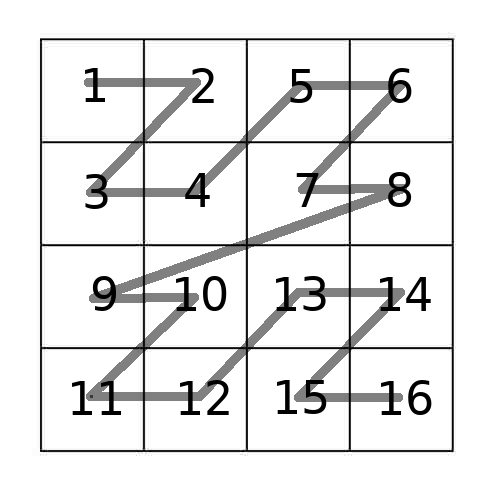
\includegraphics[width=0.3\textwidth]{img/ZCurveSpaceFillingCurve.png}
\caption{Z erdvę užpildančios kreivės pavyzdys.}
\label{img:ZCurveSpaceFillingCurve}
\end{center}
\end{figure}

Tarsime, kad erdvė $E^d$ nėra begalinė, ir $[0, 2^b]$ yra visų šios erdvės koordinačių ašių ribos.
Formaliai tvarka yra apibrėžiama sąryšio:
\begin{equation}
	p_1 < p_2 \text{ jeigu } ZCSFC(p_1) < ZCSFC(p_2)
\label{eq:ZCurveSFCComparison}
\end{equation}

Čia $p_1$ ir $p_2$ yra taškai erdvėje $E^d$, o $ZCSFC(p)$:

\begin{equation}
	ZCSFC(p) = \sum_{i=0}^{b-1} \sum_{j=0}^{d-1} [2^{i*b+j} BITSET(p_j, i)]
\label{eq:ZCurveSFCValue}
\end{equation}

Čia:

\begin{equation}
	BITSET(p, i)=
\begin{cases}
	1,& \text{jeigu } \text{i-asis bitas yra 1 skaičiaus p dvejetainėje formoje}\\
	0,& \text{kitu atveju}\\
\end{cases}
\label{eq:Bitset}
\end{equation}






\subsection{SP-GIST karkasas}
% sp-gists
% bulk operations on sp-gists
% postgre (min 3)

\input{sections/queries}
\input{sections/block_size_performance}
\input{sections/memory_management}
\input{sections/prefix_search}
\input{sections/k-d_tree}
%\sectionnonum{Rezultatai ir išvados}
%Rezultatų ir išvadų dalyje išdėstomi pagrindiniai darbo rezultatai (kažkas
%išanalizuota, kažkas sukurta, kažkas įdiegta), pateikiamos išvados (daromi
%nagrinėtų problemų sprendimo metodų palyginimai, siūlomos rekomendacijos,
%akcentuojamos naujovės).


\printbibliography[heading=bibintoc]
%\appendix

\section{Metodų skirtų daugiamačių duomenų indeksavimui apžvalga}
\label{app:multidimensionalIndexing}
\begin{figure}[H]
\begin{center}
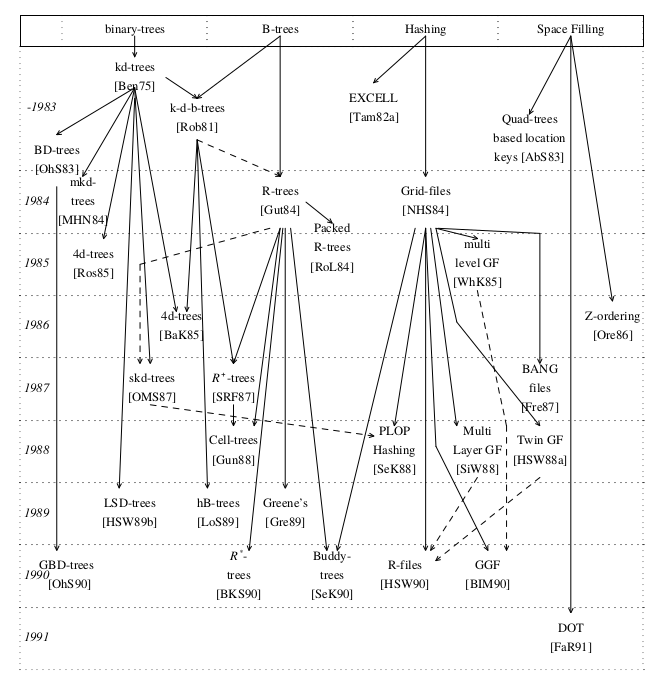
\includegraphics[width=\textwidth]{img/MultidimensionalDataIndexing.png}
\caption{\cite{bader2012space} pateikiama metodų, skirtų daugiamačių duomenų indeksavimui, schema}
\end{center}
\end{figure}

\section{Įvairių užklausų pavyzdžiai}

\label{app:pointQuery}
\begin{figure}[H]
\begin{center}
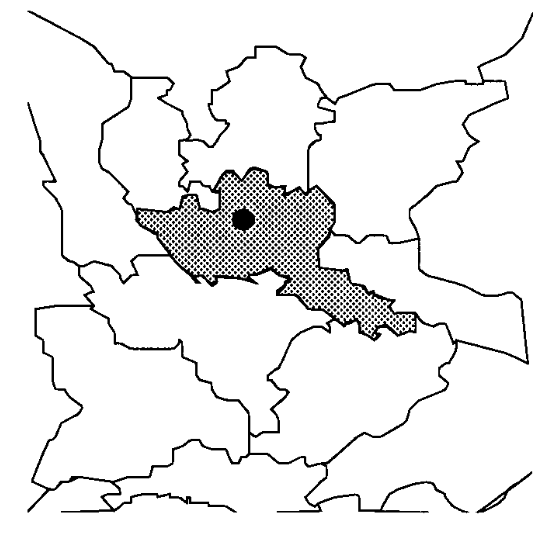
\includegraphics[width=0.4\textwidth]{img/PointQuery.png}
\caption{Taško užklausos pavyzdys}
\end{center}
\end{figure}

\label{app:windowQuery}
\begin{figure}[H]
\begin{center}
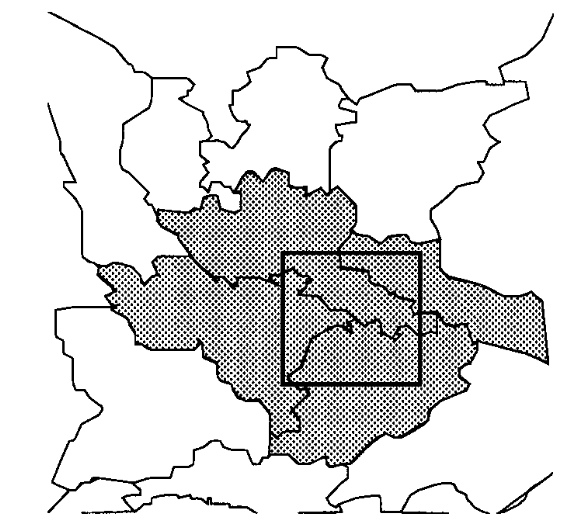
\includegraphics[width=0.4\textwidth]{img/WindowQuery.png}
\caption{Lango užklausos pavyzdys}
\end{center}
\end{figure}

\label{app:enclosureQuery}
\begin{figure}[H]
\begin{center}
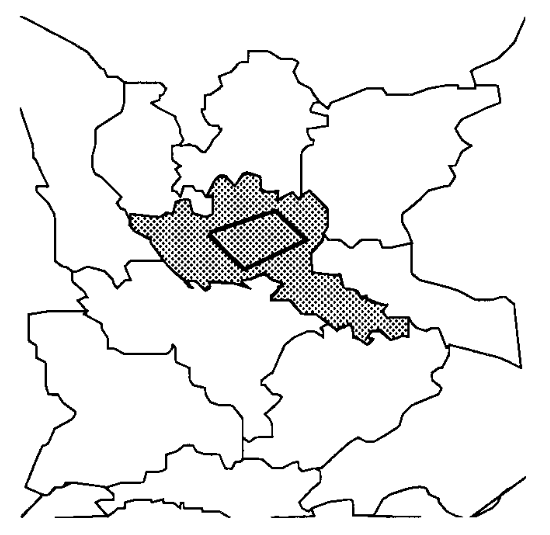
\includegraphics[width=0.4\textwidth]{img/EnclosureQuery.png}
\caption{Apgaubiančiosios užklausos pavyzdys}
\end{center}
\end{figure}

\label{app:intersectionQuery}
\begin{figure}[H]
\begin{center}
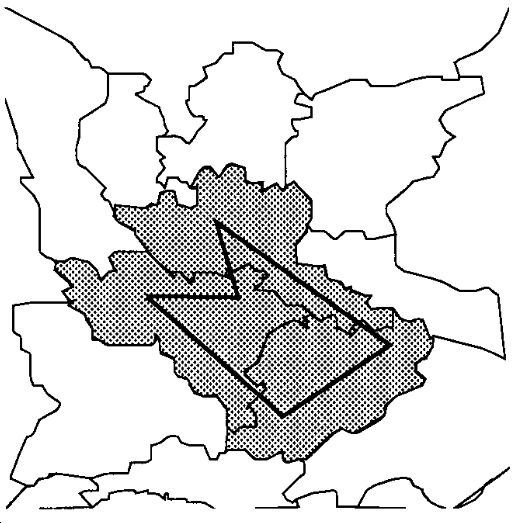
\includegraphics[width=0.4\textwidth]{img/IntersectionQuery.png}
\caption{Regiono užklausos pavyzdys}
\end{center}
\end{figure}

\label{app:containmentQuery}
\begin{figure}[H]
\begin{center}
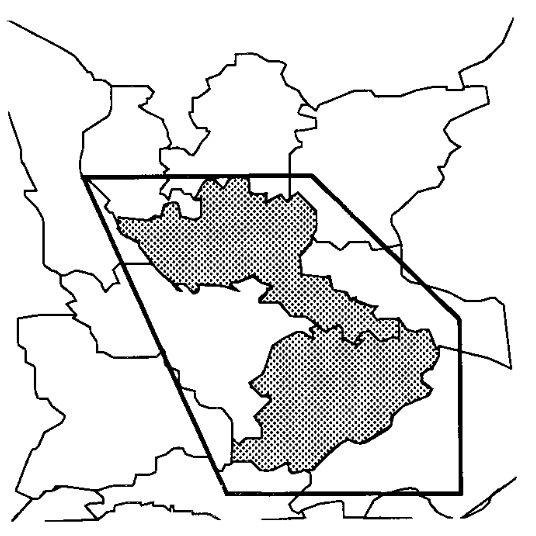
\includegraphics[width=0.4\textwidth]{img/ContainmentQuery.png}
\caption{Pilno regiono užklausos pavyzdys}
\end{center}
\end{figure}

\label{app:adjacencyQuery}
\begin{figure}[H]
\begin{center}
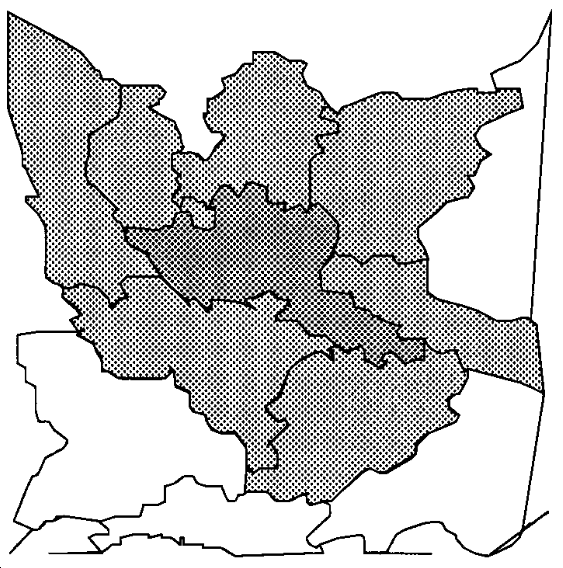
\includegraphics[width=0.4\textwidth]{img/AdjacencyQuery.png}
\caption{Kaimynų užklausos pavyzdys}
\end{center}
\end{figure}








\end{document}
